\section{Normalized Message Format}
\label{sec:normalizedmessage}

In this diploma thesis we modify the \ac{NMF} design in \cite{gomez2012}, due to the different data types which are transferred in it. Gomez presents a \ac{NMF} where the data is transferred in its body in \ac{XML} format, which suites for the communication protocols his prototype supports (SOAP, JMS, and E-mail), and the text data type contained in the requests. Furthermore, the multi-tenant aware routing supported in his approach is static between endpoints (e.g. one incoming request is routed from one tenant's consumer endpoint to one tenant's provider endpoint). The complexity of the data types transferred in the system and the dynamic routing between backend Cloud data stores leads us to modify the meta-data transported in the \ac{NMF} properties section, and to send the data in the attachment section. We are also forced to design two different data structures for the \ac{NMF}: one for request messages, and another for response messages. The data and meta-data contained in the MySQL requests and responses messages require the utilization of different data structures to transmit them in the \ac{NMF} (see Listing \ref{lst:nmfcontent}). MySQL requests contain user, authentication, etc. meta-data, while the MySQL response contain meta-data which describes the data transferred. 

\begin{figure}[htb]
	\centering
		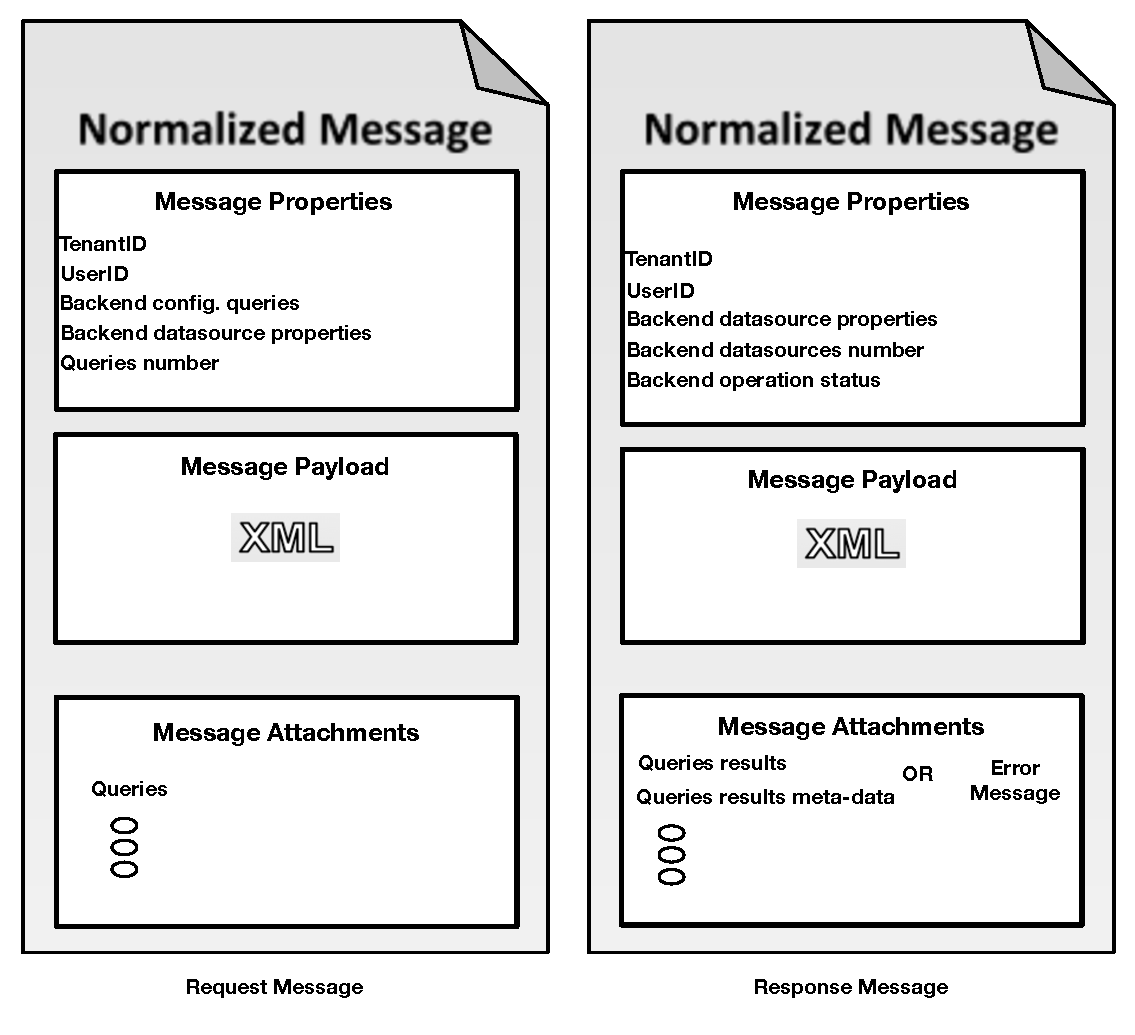
\includegraphics[clip, scale=0.7]{./gfx/normalizedMessage.pdf}
	\caption[Normalized Message Format Design]{Design of the Normalized Message Format used in the system.}
	\label{fig:nmf}
\end{figure}

Data access or modification requests to backend data stores through ServiceMix-mt are received in the vendor's communication protocol, e.g. MySQL communication protocol for MySQL database systems, or \ac{JSON} over \ac{HTTP} for \ac{NoSQL} databases, must be marshaled to the \ac{NMF} structure. The \ac{NMF} sections we use for incoming requests are the message properties, and the message attachment (see Figure \ref{fig:nmf}). In the message properties we attach tenant context information (tenant and user \ac{UUID}), and the request's meta-data, which is divided into:
	\begin{itemize}
		\item Backend configuration queries: server configuration queries sent prior to the request query, e.g. setting the predefined language, character encoding, etc. These must be executed in the backend database system, and are sent to the backend database system prior to the request query.
		\item Backend data source properties: in this property structure the set of backend data sources meta-data are stored, e.g. access credentials, main (and secondary) information structures names, data source type, etc.
		\item Queries number: the number of queries which are sent as attachment. The default value is one, but in multi-querying this value increases.
	\end{itemize}  

The \ac{NMF} body supports text data format. The data transferred to or retrieved from a backend Cloud data store is represented as different data types, e.g. string, integer, float, binary, etc., and must be transferred as binary data. Therefore, the queries contained in the user's requests are sent in the attachment section of the \ac{NMF}, which supports objects serialization. The queries are stored in a vector structure which can contain multiple queries. The \ac{NMF} request must be demarshaled to the appropriate database system's communication protocol before forwarding the user's request to the backend database system. 

Responses from the backend data stores are correlated with the user's request, marshaled, and sent back in the response \ac{NMF} (see Figure \ref{fig:nmf}). Data retrieved from a data store, e.g. in a data retrieval or update operation, contains both data and meta-data. Both informations are stored in vector structures in the attachment section of the response \ac{NMF}. In case of error, the error message is stored in the response \ac{NMF}, and forwarded back to the user. In the message properties section the tenant context information (tenant and user \ac{UUID}) is stored, and the response meta-data, which contains the following information:
	\begin{itemize}
		\item Backend data source properties: in this property structure the set of backend data sources meta-data are stored, e.g. main (and secondary) information structures names, data source type, etc.
		\item Backend data source number: the number of targeted data stores. 
		\item Backend operation status: the overall operation status. We consider operations over one or more target data stores as atomic. If one or more backend data stores returns an error, the operation status is set to error, and an error is forwarded back to the user. 
	\end{itemize}  

The message body may be used for sending structured data in \ac{XML} format. However, we do not send information in this \ac{NMF} section in this diploma thesis, due to the need to transfer the requests and response data as binary serializable objects (serializable vectors) in order to avoid errors in the data content if the data is transformed to string, and structured in XML format. 
\FloatBarrier